\documentclass[12pt,a4paper,onecolumn]{article}
\usepackage[margin=27mm]{geometry}
\usepackage{fontspec,xeCJK,amsmath,graphicx}
\setmainfont[Path=C:/Windows/Fonts/,BoldFont=timesbd.ttf]{times.ttf}
\setCJKmainfont[Path=C:/Windows/Fonts/,BoldFont=kaiu.ttf]{kaiu.ttf}
\renewcommand{\normalsize}{\fontsize{12bp}{18bp}\selectfont}
\setlength{\parindent}{2em}
\setlength{\parskip}{5bp}
\newcommand{\captionline}[1]{\par\noindent #1\par\smallskip}
\begin{document}
\normalsize
\noindent\textbf{階段 I｜正文示範}\par
\section*{JPEG 壓縮對影像奇異值與低秩結構之影響分析}

先看欄杆與後方的灰牆。左邊是原圖，中間和右邊是同一原圖分別以 Q=40、Q=95 編碼後的解碼圖。這個窗口保留了共同的輪廓，光看縮圖卻很難判斷整張影像的像素差了多少。

\noindent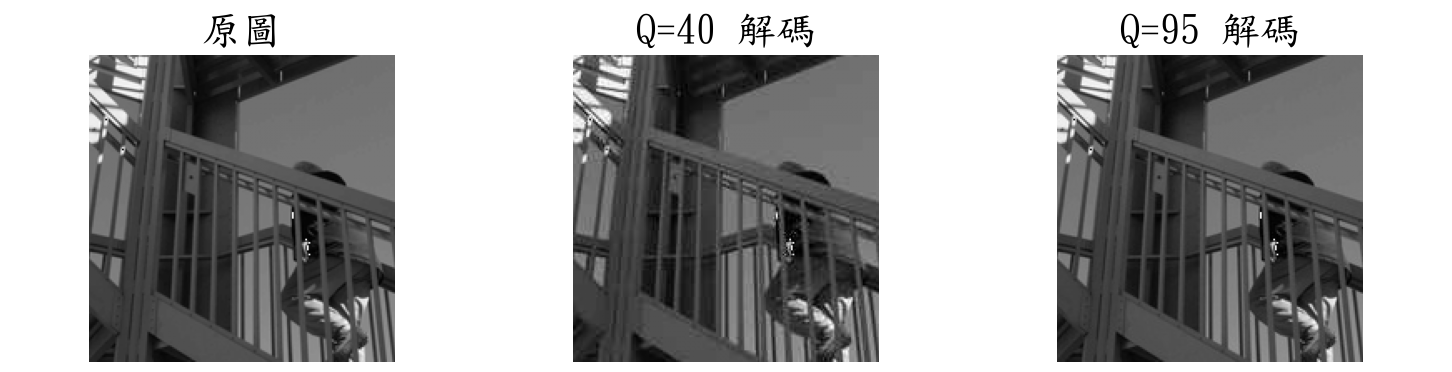
\includegraphics[width=\linewidth]{reports/stage-i/jpeg-crops.png}
\captionline{圖 1．原圖與兩張實際解碼圖的同位置裁切。三格使用相同灰階範圍，取自 M2 存檔。}

圖 2 上半部用峰值訊雜比（PSNR）量化整張解碼圖與原圖的差異。Q=40 為 32.44 dB，低於 Q=95 的 46.03 dB。下半部卻出現反差：若每張解碼圖都只保留自己的前 100 個成分，Q=40 的相對平方誤差是 0.46522\%，比 Q=95 的 0.52482\% 小。

\noindent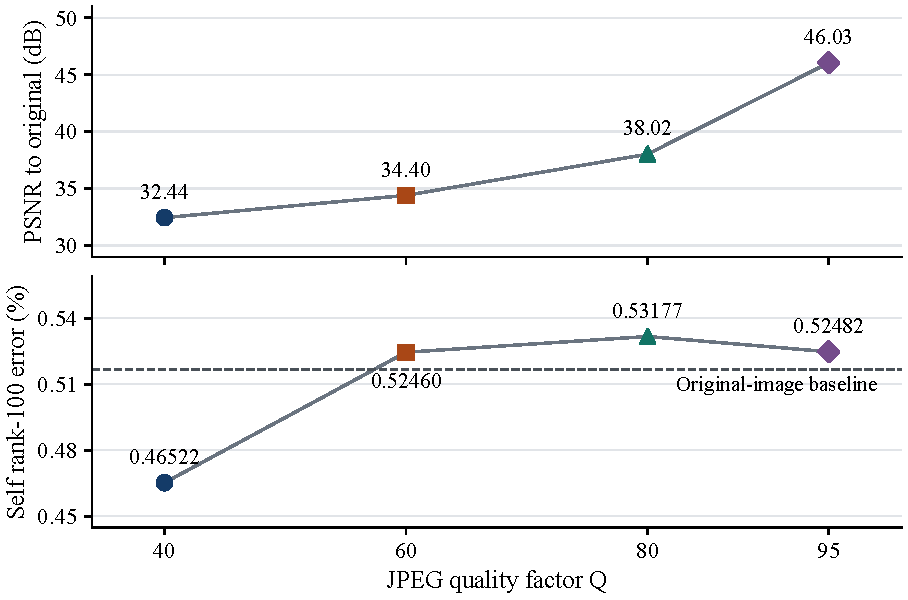
\includegraphics[width=\linewidth]{reports/stage-i/COMPARISON.pdf}
\captionline{圖 2．上圖以原圖為參照，下圖以各解碼圖自身為參照。虛線是原圖自身的 Rank-100 相對平方誤差，獨立於四個 JPEG 資料點。來源為 M2 的 \texttt{jpeg\_metrics.csv} 與 \texttt{rank\_errors.csv}（$k=100$）。}

Q=40 雖然離原圖較遠，卻能用同樣數量的成分更接近它自己。要弄清楚這個反差，得先看看只保留少數成分時，欄杆會變成什麼樣子。

\newpage
\section*{一個成分能畫出多少欄杆？}

圖 3 的四張重建都來自原圖，只改變保留項數。保留一項時，局部大致只剩成帶的亮暗變化。到十項時可看出欄杆的走向，但相鄰細線仍容易連成一片。保留五十及一百項後，線條與間隙逐步分開。

\noindent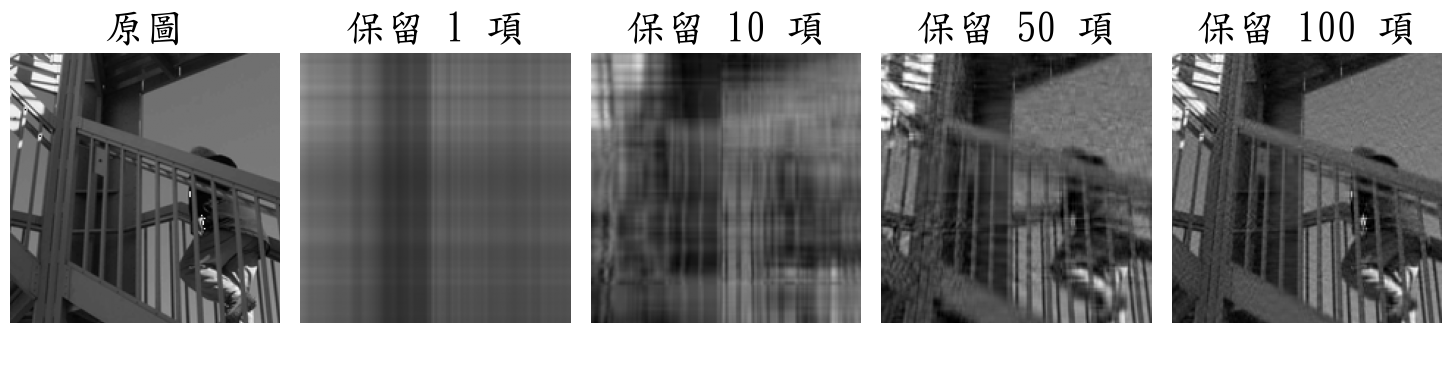
\includegraphics[width=\linewidth]{reports/stage-i/rank-crops.png}
\captionline{圖 3．原圖與既有 Rank-1、10、50、100 重建的同位置裁切。五格採同一灰階範圍，截斷過程未經 JPEG 編碼。圖像取自 M2 存檔。}

為什麼只保留一項時，斜欄杆的形狀不見了？想像用一條橫向輪廓 $[1,3]$ 畫兩列。第一列照畫，第二列全部乘二。直向權重乘上橫向輪廓，結果就是外積：
\begin{equation}
 \begin{bmatrix}1\\2\end{bmatrix}
 \begin{bmatrix}1&3\end{bmatrix}
 =\begin{bmatrix}1&3\\2&6\end{bmatrix}.
\end{equation}
兩列亮度不同，左右的比例始終是 $1:3$。若斜欄杆在下一列往右移，光把整列乘上一個常數無法移動亮點。疊加其他形狀的外積，才能在不同位置增減亮度。

奇異值分解（SVD）讓我們把這種疊加用在整張影像。令 $X$ 是正在分析的像素矩陣。第 $i$ 個外積由直向向量 $u_i$ 和橫向向量 $v_i$ 組成，權重 $\sigma_i$ 為奇異值，按非遞增順序排列。$p$ 是矩陣的列數與欄數中較小者。原圖的加總截到第 $k$ 項，就是圖 3 的重建操作：
\begin{align}
 X &= \sum_{i=1}^{p}\sigma_i u_i v_i^{\mathsf T},\\
 X_k &= \sum_{i=1}^{k}\sigma_i u_i v_i^{\mathsf T}.
\end{align}
欄杆的外觀指出差在哪裡。要比較整張圖少了多少，則要把這些局部差異加總。

\newpage
\section*{兩個誤差，各自和誰比較？}

把原圖換成品質因子 $Q$ 的解碼圖 $B_Q$，前一頁的截斷操作仍然成立。把影像減去它自己的截斷重建，差圖只剩沒保留的成分。左右奇異向量各自正交歸一，因此外積方向也在 Frobenius 內積下正交，且長度為一。以 Frobenius 範數將差圖的像素平方加總時，交叉項為零，所以對任一影像 $X$，
\begin{equation}
 \lVert X-X_k\rVert_F^2=\sum_{i>k}\sigma_i^2 .
\end{equation}
在秩不超過 $k$ 的候選中，截斷 SVD 的 Frobenius 誤差最小。兩張圖的總平方能量可以不同，因此圖 2 下半部對各非零矩陣另除以自身總平方能量：
\begin{equation}
 R_k(X)=\frac{\lVert X-X_k\rVert_F^2}{\lVert X\rVert_F^2}
       =\frac{\sum_{i>k}\sigma_i^2}{\sum_i\sigma_i^2}.
\end{equation}
Q=40 的 0.46522\% 比 Q=95 的 0.52482\% 小，表示用各自的前 100 項重建時，Q=40 未保留的平方能量占比更小。

PSNR 的計算不做截斷。令 $A$ 為原圖，$m,n$ 為影像的列數和欄數。先算解碼圖與原圖的逐像素均方差，再以 8 位元灰階峰值 255 換算為 dB：
\begin{align}
 \operatorname{MSE}(A,B_Q)&=\frac{\lVert A-B_Q\rVert_F^2}{mn},\\
 \operatorname{PSNR}(A,B_Q)&=10\log_{10}\!\left(\frac{255^2}{\operatorname{MSE}(A,B_Q)}\right).
\end{align}
均方差為零時，PSNR 為無限大。Q=40 的 32.44 dB 低於 Q=95 的 46.03 dB，表示前者偏離原圖較多。兩項結果可以同時成立：解碼圖離原圖更遠，仍可能更容易描述它自己。較低的自身誤差無法證明它留下更多原圖細節。這項觀察限於同一張圖和四組編碼設定。

兩把尺都把全圖差異壓成一個數字。若想追蹤原圖的某個秩一成分在解碼後如何改變，能否讓四張解碼圖始終用原圖的方向來比較？
\end{document}
